\section{Introduction}\label{sec:intro}
JavaScript is the de facto programming language in web development and,
moreover, blossoming beyond the web.
JavaScript has dominated client-side scripting of the web for over a decade.
JavaScript takes the unique position as the universal language operating in both
the browser and on a server in the form of Node.js.
The client-side frameworks such as React, Vue.js, and Angular have accelerated
the universal use of JavaScript.
The cross-platform frameworks like React Native and Electron have spread
JavaScript to the new domains of mobile and desktop beyond the web.
This is only possible thanks to JavaScript's easy operation in development and
deployment with scripting language characteristics such as dynamic and
interpreted language features~\cite{weaklySPE}.


However, such features make it difficult to support developer tools that require
statically reasoning about semantics of JavaScript programs such as call graph
construction, type checking, optimization, and bug detection.
For example, the combination of the JavaScript features: dynamically-computed
property name, prototype chain, and first-class function, makes call graph
construction challenging.
Even a minor precision loss at property name can cause reading all methods in
the object and its prototype chain, including hundreds of built-ins, that
results in useless analysis results.
In static analyses of Java, the benchmark results clearly show the trade-off
between precision and performance~\cite{introspective, data-driven}, a low degree of
context sensitivity shows a high performance but low precision.
In the case of JavaScript, the relationship between precision and performance is
more complex due to the spurious callee explosion.
Low precision tends to cause the large number of spurious callees, which
significantly degrades the performance~\cite{correlation, determinacy-jQuery, weaklySPE, value-refinement}.


For this reason, recent studies on JavaScript static analysis have developed
to improve analysis precision against this challenge.
Madsen et al.~\cite{string, regex, combining-string} presented sophisticated abstract domains for strings.
Park et al. proposed higher degrees of context sensitivity for loops~\cite{lsaECOOP, lsaSPE}.
Relations between object properties have aided to analysis precision~\cite{correlation, weaklyAPLAS, weaklySPE}.
The idea stretches from property name to non-local variables and types for predicate functions~\cite{value-partitioning}.
The on-demand backward analyses~\cite{value-refinement} refines imprecise values for property writes.


Unfortunately, it does not mean that high precision leads to "good" performance
but "better" than the "bad" performance.
Computation costs of high degree of sensitivity remains as it is but the
snowball of low precision is much larger than that.
We alleviate computation costs of high degrees of sensitivity through a combined
approach of static and dynamic analyses.


Existing combined approaches derive three kinds of benefits of dynamic analysis.
Dynamic analyses~\cite{jalangi, dlint} can run on a highly-optimized
JavaScript engine like V8, so it can boost up analysis performance.
There is no precision loss coming from limitations of abstract domains and
sensitivities if the dynamic analysis terminates~\cite{determinacy, concerto}.
Dynamic analysis can pass by opaque codes that require extra handling for static
analysis~\cite{battles, sra}.

However, the existing combined analyses are limited to maximize benefits of
dynamic analysis.
Staged analyses first collect particular information by dynamic analysis and
apply static analysis augmented with dynamic information~\cite{blendedJava, eha}.
Dynamic information can be determinacy facts~\cite{determinacy}, call graphs~\cite{tunable}
object creation site~\cite{blendedJS}, or entire heap at specific program points~\cite{battles}.
Once static analysis starts, it does not utilize more dynamic information.
The other design of combined analysis is divide whole program into two parts~\cite{concerto}.
One (framework code) for the dynamic analysis  and the other (user code) for the
static analysis.
The policy to divde a program is predefined and syntactic and never changes
during analysis.


We present a more flexible and fine-grained method to combine two analyses to
maximize benefits.
Our approach extend dynamic analysis to work with the presence of abstract
values, named lazy concrete execution.
The analysis goes on a concrete engine side as much as possible until
non-determinism is actually introduced by abstract values or analysis
sensitivity that the lazy concrete execution cannot handle.
When the lazy concrete exeuction meets non-determinism, the analysis switches to
the traditional static analysis and uses its abstract semantics to handle that.
As soon as analysis sensitivity is deterministic, it switches to the lazy
concrete execution again.

\begin{figure}
  \centering
  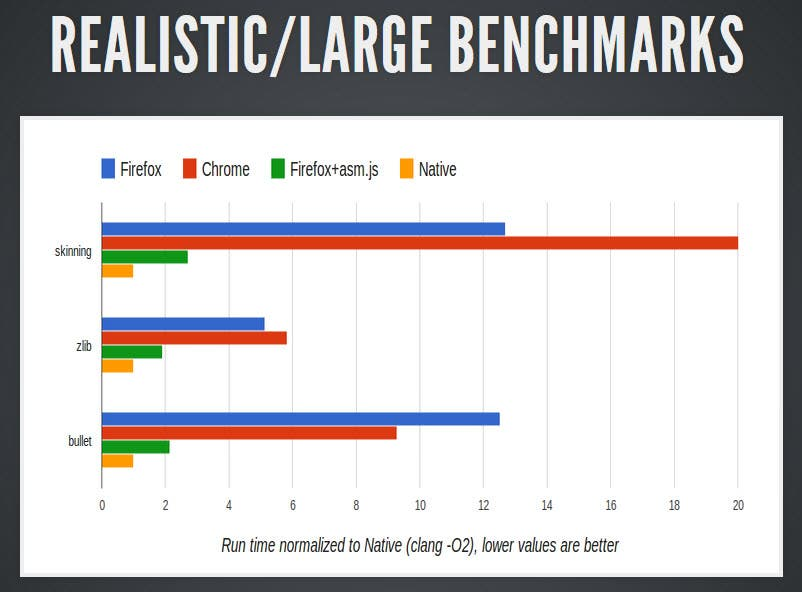
\includegraphics[width=\linewidth]{benchmark_performance}
  \caption{The performances of static and dynamic analyses on deterministic benchmarks}
  \label{fig:performance}
\end{figure}

Our key observation is that high degrees of sensitivity increase the use of
concrete semantics during analysis and utilizing an optimzied engine like V8 is
the fast way to apply concrete semantics.
As shown in Figure~\ref{fig:performance}.
Our design is not limited to any predefined features including program point and
does not harmful to the soundness of the original static analysis.


%We have demonstrated how dynamic shortcut maximize benefits of dynamic analysis.
%We have implemetned our method by extending the existing JavaScript static
%analyzer.
%We found that using dynamic shortcut significantly increased performance for
%benchmark programs enhanced with abstracted input.

In summary, the contributions of this paper are as follows.
\begin{itemize}
\item We formally describe the high-level idea of adding dynamic shortcuts, a
  technique for combining static and dynamic analyses into fine-grained level on
  the general abstract interpretation framework (Section 3).
  We explain JavaScript related details formalized with core language of JavaScript as well (Section 4).
\item We actualize our method by extending the existing JavaScript static analyzer SAFE 2.0.
  We explain key techniques to synchronize two analyses (Section 5).
\item We empirically evaluate our technique using the implementation (Section 6).
  We find that using dynamic shortcut significantly increased performance for
  benchmark programs enhanced with abstracted input that existing combined
  analysis designs cannot handle.
\end{itemize}

%There are almost 200 million active websites out of over 1.8 billion sites on the entire web.
%https://www.internetlivestats.com/total-number-of-websites/
%JavaScript is used as client-side programming language by 96.9\% of all the websites.
%https://w3techs.com/technologies/history_overview/client_side_language/all/y
